\section{Structured Query Language Databases}
\label{sec:fundamentalssql}  

The \ac{SQL} stands nowadays as the standard computer database language in \ac{SQL} \ac{DBS}. \ac{SQL} is a tool for organizing, managing, and retrieving data stored by a computer database \cite{sql1999}. The \ac{SQL} language is nowadays one of well known languages in the IT sector. Thus, we introduce in the following sections in the \ac{SQL} \ac{DBS} and their specific communication protocol we use in this thesis, rather than on the language they support. 

The final prototype of this diploma thesis aims to provide support for most of the \ac{DBS} communication protocols available in the market. However, we crashed into vendor-specific communication protocol implementations along the available \ac{DBMS} in the market, rather than a common standardized communication protocol. For this reason, we provide support for incoming connections which comply the MySQL \ac{DBS} communication protocol and give the hints for supporting the PostgreSQL \ac{DBS} communication protocol. However, for outgoing connections we have not found such problem, due to the management of the different vendor's native drivers provided by \ac{JDBC}, which is introduced at the end of this section. 

\subsection{MySQL Database System}
MySQL is nowadays the most popular Open Source SQL \ac{RDBMS} \cite{mysqlmanual}. Data is stored following a relational storage model, where data is represented as tuples, and grouped into relations. The main storage structure managed in this type of database are tables, which can be linked together by establishing relationships governed by rules, e.g. one-to-one, one-to-many, many-to-many, etc. 

The MySQL server is one of the main components in the \ac{DBMS}. It is a client/server system which consists of a multi-threaded SQL server which supports different backends, several different client programs and libraries, administrative tools, and a wide range of application programming interfaces (APIs) \cite{mysqlmanual}. Its main functionality we discuss in this diploma thesis is the protocol it supports for I/O operations between the client and the server. The MySQL communication protocol has changed over time and over the \ac{DBMS} version upgrades, leading to different new user authentication methods, new data types, etc. In this diploma thesis we cover the MySQL versions 5.x support. Due to the compatibility of the native \ac{JDBC} drivers along the different versions, the supported protocol in our prototype is full compatible with the last released \ac{JDBC} MySQL native driver.

The MySQL communication protocol is used between the MySQL client and server. Implementations of the protocol can be found in the MySQL server, the MySQL native driver Connector/J (Java implemented) and in the MySQL proxy. As it is described in Figure \ref{fig:mysqlprotocol}, the whole communication process between a MySQL client and a MySQL server is divided into three phases: connection phase, authentication phase, and command phase, and their main transferred information unit are MySQL packets. The MySQL packet configuration and the supported data types are described in Chapter \ref{chap:implementation}.

\begin{figure}[htb]
	\centering
		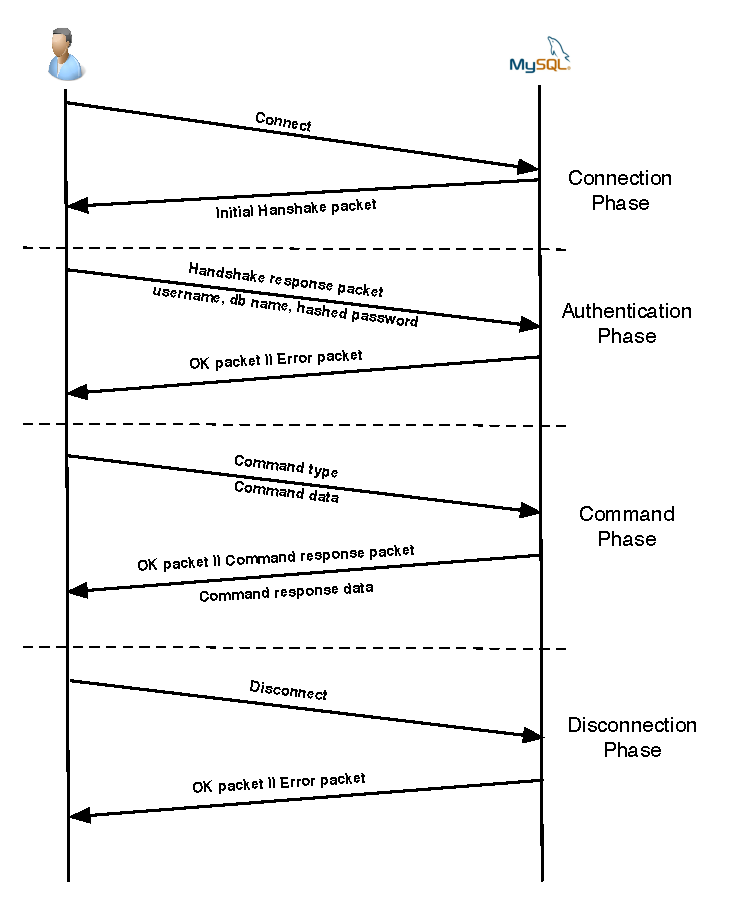
\includegraphics[clip, scale=0.8]{./gfx/mysqlprotocol.pdf}
	\caption[MySQL Communication Protocol]{MySQL communication protocol in the four communication phases \cite{mysqlmanual}}
	\label{fig:mysqlprotocol}
\end{figure}

During the connection phase, the client connects via \ac{TCP} to the port where the main MySQL server thread listens on (commonly used port 3306). In the connection and authentication phases, the MySQL server sends to the client an initial handshake packet, containing information about the server, server flags, and a password challenge. The client responds with his access credentials and communication configuration flags. When the authentication succeeds, the command phase is initiated. This phase is actually where the operations on the database or on the server take place, e.g. server configuration, querying, statements execution, etc. The connection between the client and the server must be always ended in the client side, except for internal errors in the server where the communication is interrupt and lost. 

In this diploma thesis we extend a Java implementation of the MySQL protocol, which is described in more detail in Chapter \ref{chap:relatedworks}, and adapt it for its integration and communication in ServiceMix-mt.

\subsection{PostgreSQL Database System}

PostgreSQL is known as an \ac{ORDBMS}. An \ac{ORDBMS} is quite similar to the a \ac{RDBMS} model explained in the last section, but its main difference is that it also supports the object-oriented database model, where objects are stored in database schemas can be accessed using the \ac{SQL}. 

The PostgreSQL \ac{DBMS} also implements a client/server model for its I/O operations in the database. In contrast to the MySQL server, the PostgreSQL server defines the following cycles depending on the state of the connection: start-up, query, function call, copy, and termination \cite{postgresqlmanual}. During the start-up phase, the client opens a connection and directly provides its user name and the database he wants to connect. This information identifies the particular protocol version to be used. The server responds with an authentication challenge which the client must fulfill. 

The MySQL's SQL command phase is in this server denoted as a query cycle. A query cycle is initiated with the reception of an SQL command, and terminated with the response of the query execution. 

The function call cycle allows the client with execute permissions to request a direct call of an existing function in the system's catalog. The copy cycle switches the connection into a distinct sub-protocol, in order to provide a high-speed data transfer between the client and the server. 

The termination of a successful or failed client/server communication is handled in the termination cycle, which involves the transfer of a termination packet from the client to the server in the successful case, and from the server to the client when the termination is due to a failure. 
 
\subsection{MySQL Proxy}

The MySQL Proxy is an application which supports the MySQL communication protocol between one or more MySQL clients and MySQL servers \cite{mysqlproxy}. In a distributed storage system where different clients connect to different servers a proxy which acts as a communication intermediary may significantly increase the overall performance. The MySQL proxy supports communication management between users, communication monitoring, load balancing, transparent query alteration, etc. Oracle releases a MySQL proxy which supports MySQL 5.x or later, and implemented in the C programming language. 

Integrating a MySQL server into a \ac{ESB} collisions with the main concept of an \ac{ESB} as an intermediary technology between services. For this reason, in this diploma thesis we integrate and extend a Java version of a MySQL proxy developed by Continuent Inc.: Tungsten Connector \cite{tungstenwiki}.

\subsection{Java Database Connectivity}

\ac{JDBC} is widely used in the connection to databases in the Java programing language. JDBC technology allows programers to use the Java programming language to exploit "Write Once, Run Anywhere" capabilities for applications that require access to enterprise data.\cite{jdbcspec}. Its management of different vendor-specific native drivers allows businesses not to be locked in any proprietary architecture, but to be able to connect to different databases simply by specifying the driver's name and the connection properties in the \ac{JDBC} URL. 

The \ac{JDBC} Driver Manager or DataSource Object implements the selection of the appropriate vendor's native driver specified in the \ac{JDBC} URL. However, the vendor's native driver must be installed prior to execution. 

In this diploma thesis we take advantage of this technology in order to enable our final prototype to support a multi-protocol database outgoing communication (from the prototype to external \ac{DBS}).  


\FloatBarrier
